% % Primera página del documento
\begin{titlepage}
    \begin{scriptsize}\noindent Facultad de Informática.\\
        Ingeniería en Informática.\\
        Ingeniería del Software.\\
        Proyecto: Everywhere House Control.
    \end{scriptsize}\\
    \vfill
    \begin{center}
        \begin{Large}
            \textbf{Documento de disenño}
        \end{Large}
    \end{center}
    \vfill
    \begin{flushright}
        \begin{scriptsize}
            \begin{tabular}{lll}
            Creado por & Gutierrez, Hector & Guzman, Fernando  \\
                 & Ladrón, Alejandro & Maldonado, Miguel Alexander \\
                 & Morales, Álvaro & Ochoa, Victor \\
                 & Rey, José Antonio & Saavendra, Luis Antonio  \\
                 & Tirado, Colin & Vicente, Victor \\
            \end{tabular}
        \end{scriptsize}
    \end{flushright}
\end{titlepage}
\thispagestyle{empty}
\cleardoublepage
\newpage

% % Tabla de contenidos, etc.
\pagenumbering{Roman}
\tableofcontents
\newpage
\thispagestyle{empty}
\cleardoublepage
\newpage
\pagenumbering{arabic}
\raggedbottom
\interfootnotelinepenalty 10000

\chapter{Introducción}
\section{Propósito}
El objetivo de este documento es la de mostrar, de una forma más específica, el funcionamiento del sistema en los distintos entornos en el que se desarrolla /textitt{EHC}. 
\section{Alcance}
El contenido de este documento detallada las decisiones tomadas en cuanto a la arquitectura del sistema y los casos de uso que deberá satisfacer el producto una vez concluido el desarrollo de este.
\section{Definición, acrónimos y abreviaciones}
Ver glosario en el documento <Tenemos que hacer el doc del glosario y abreviaciones>
\section{Referencias}
Citar a los otros documentos, SRS, Planificacion....
\section{Vista general}
Sección candidata a ser borrada o poner la estructura general del documento, como un índice
\chapter{Representación del sistema}
En este documento, se describen las distintas arquitecturas adoptadas para realizar un sistema que cumpla con los requisitos solicitados con la máxima calidad posible. Podemos representar el sistema como un conjunto de los siguientes componentes:
 \begin{itemize}
 \item Vista de casos de uso: donde se presentan los actores y los casos de uso para el sistema donde se manifiesta lo que percibe los distintos actores en distintas situaciones del sistema. 
 \item Vista lógica: se detallan los requerimientos funcionales y podemos observar como puede funcionar el sistema a través de diagramas entidad-relación y diagramas de clase.
 \item Vista de procesos: en esta componente, nos centramos en otros aspectos del sistemas más enfocados al rendimiento y disponibilidad del sistema. Algunos de los temás tratados son la concurrencia, distribución e integridad del sistema.
 \item Vista de despliegue: en esta vista nos centramos más en mostrar la arquitectura hardware del sistema. Debido al uso de distintos componentes hardware y a sus respectivas interfaces, esta vista se convierte en una de las principales vistas que define el sistema.
 \item Vista de implementación: describe la estructura general del modelo de implementación, distribución del software y la interrelación entre sus partes.
 \end{itemize}

\chapter{Objetivos y restricciones}

\section{Del software}

La comunicación de la aplicación EHC está basada en la arquitectura Cliente-Servidor que define una serie de requerimientos claves y restricciones del sistema. 

La conexión entre la aplicación y los distintos elementos hardware que componen el sistema deben de estar garantizada. Esta comunicación es vital para el usuario, pero existe una serie de requisitos que deben cumplirse seg\'un el ámbito en el que se encuentre:
\begin{itemize}
\item Si se accede a la aplicación en el entorno EHC: la aplicación debe conectarse vía red local con el servidor local instalado en la Rasperry.
\item Si se accede a la aplicación fuera del entorno EHC: la aplicación debe conectarse vía Internet con el servidor externo para tener control a los elementos instalados en el entorno EHC
\end{itemize}

Además de estos requisitos de comunicación de la aplicación EHC, el sistema debe ...
\begin{itemize}
\item ... ser capaz de atender una alta carga de trabajo de las peticiones solicitadas por los usuarios del sistema.
\item ... proveer unas ciertas medidas de seguridad para garantizar el control del entorno EHC solo por aquellas personas autorizadas a ello, garantizar la integridad de los mensajes enviados, evitar la suplantación de identidad...
\item ...
\end{itemize}

\section{Del hardware}
Se debe de cumplir una serie de requisitos y restricciones para los componentes hardware que componen el sistema.
\begin{itemize}
\item Cada componente del entorno EHC debe de encontrarse en unas medidas óptimas de ambiente (es decir, temperatura, humedad, radiación solar...) definidas seg\'un el elemento quue sea.
\item El sistema necesita una fuente de energía constante, y si es posible, un sistema alterno que suministre energía por si la fuente principal sufre alg\'un percance. Se recomienda este sistema para que el sistema no se vea afectado con alg\'un corte de energía y así con este sistema poder apagarlo de forma segura.
\item Respetar la distancia y localización de los dispositivos con inflarrojos u otras tecnologías de transmisión directa de datos para así garantizar el correcto funcionamiento de estos dispositivos. 
\end{itemize}
\chapter{Vista de casos de uso}
\section{Introducción}
En esta vista nos disponemos a detallar varios casos de uso que pertenecen al sistema. Estos casos de uso son simplemente una descripción del comportamiento del sistema tal y como lo verían todos los usuarios participantes.

\section{Actores}
El sistema lo compone los siguientes usuarios:
\begin{description}
\item[Administrador] Este tipo de usuario es el encargado de crear/inicializar/eliminar los distintos entornos EHC y dispositivos.
\item[Super usuario] Este usuario es introducido en una configuración inicial por el \textit{Administrador}. El control en su entorno EHC es total, y también tiene el suficiente poder para crear distintos tipos de usuarios para los participantes del entorno EHC con unos distintos privilegios definidos por este. 
\item[Usuario] Es un tipo de usuario creado por el \textit{Super usuario}. Su funcionalidad depende de los privilegios otorgados por su creador, que puede ser desde un simple \textit{Usuario} con funciones de consulta hasta un \textit{Usuario} que pueda manipular y controlas los dispositivos del entorno EHC.
\end{description}

A través de la siguiente figura mostramos un esquema general de la organización de los actores del sistema:

\begin{center}
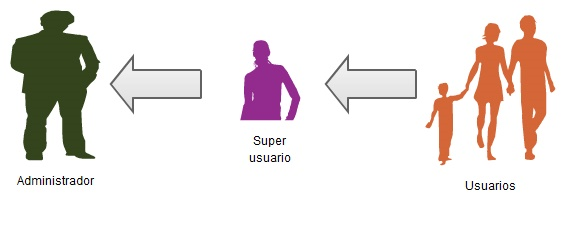
\includegraphics[width=0.7\textwidth]{4.Disenio/Imagenes/Actores}
\end{center}



\section{Casos de uso}
\subsection{Visión general de los casos de uso}
En esta sección se representan las funcionalidades y comportamientos del sistema dependiendo del tipo de usuario que se encuentre en el entorno. Gracias al estudio de los requisitos del sistema, hemos obtenido los casos de uso del sistema de una forma en la que así se agiliza el diseño del sistema y por lo tanto, su posterior implementación.
 
Mostramos a través de las figuras ~\ref{fig:cuSuperusuario} y ~\ref{fig:cuSuperusuario} los diagrama de casos de uso tanto del \textit{Super usuario} como del \textit{Administrador}. Evitamos incluir el diagrama del \textit{Usuario} ya que el \textit{Super usuario} es una extensión de este.

\begin{figure}[h!]
	\centering
	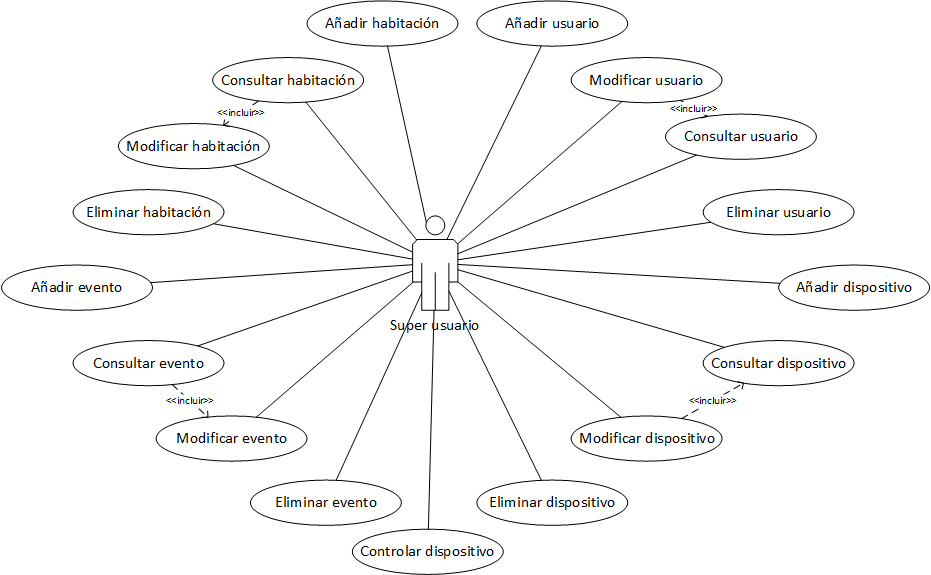
\includegraphics[width=0.7\textwidth]{4.Disenio/Imagenes/CU-Superusuario}
	\caption{Casos de uso del super usuario.}
	\label{fig:cuSuperusuario}
\end{figure}

\begin{figure}[h!]
	\centering
	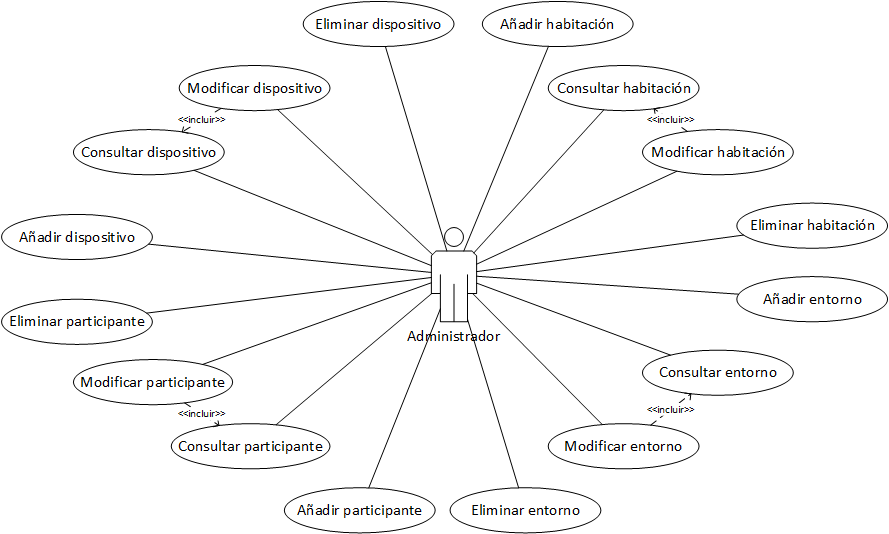
\includegraphics[width=0.7\textwidth]{4.Disenio/Imagenes/CU-Admin}
	\caption{Casos de uso del administrador.}
	\label{fig:cuAdmin}
\end{figure}


\subsection{Casos de uso en detalle}
Debido a la gran cantidad de casos de uso que hemos analizado en el sistema, la información detallada de cada uno de los casos de uso,o comúnmente conocido como \textit{Vista de escenarios}, están localizados en el documento de \textit{Casos de uso}.
\chapter{Vista l\'ogica}
\section{Introducci\'on}
Muestra los componentes principales de dise\~no del sistema y sus relaciones de forma independiente de los detalles tecnicos y de c\'omo la funcionalidad ser\'a implementada. Describiremos esta vista a trav\'es de clases, paquetes, casos de uso y subsistemas.
\section{Principales paquetes de dise\~no}

La aplicaci\'on EHC se descompone en grandes paquetes: [MIRAR ESTOS PUNTOS, NO ME CONVENCEN PARA NADA]
\begin{enumerate}
\item Presentaci\'on: Los usuarios acceder\'an al sistema a trav\'es de diferentes plataformas pero con la misma funcionalidad. Estas plataformas son:
\begin{enumerate}
\item Web: podr\'an acceder a trav\'es de cualquier ordenador con conexi\'on local (si se encuentra en el entorno EHC) o por Internet.
\item M\'ovil: dispondr\'an tanto de una aplicaci\'on para iOS como para Android.
\end{enumerate}
\item Aplicaci\'on: en este paquete englobamos todo aquello a la l\'ogica de la aplicaci\'on. Este paquete engloba:
\begin{enumerate}
\item La propia aplicaci\'on que se encarga de la propia l\'ogica de la aplicaci\'on y de operaciones sencillas.
\item Servidor: se encarga ser el enlace entre el dispositivo m\'ovil o p\'agina web y el entorno EHC.
\end{enumerate}
\item Datos: Base de datos en la nube.
\end{enumerate}

\begin{figure}[h!]
	\centering
	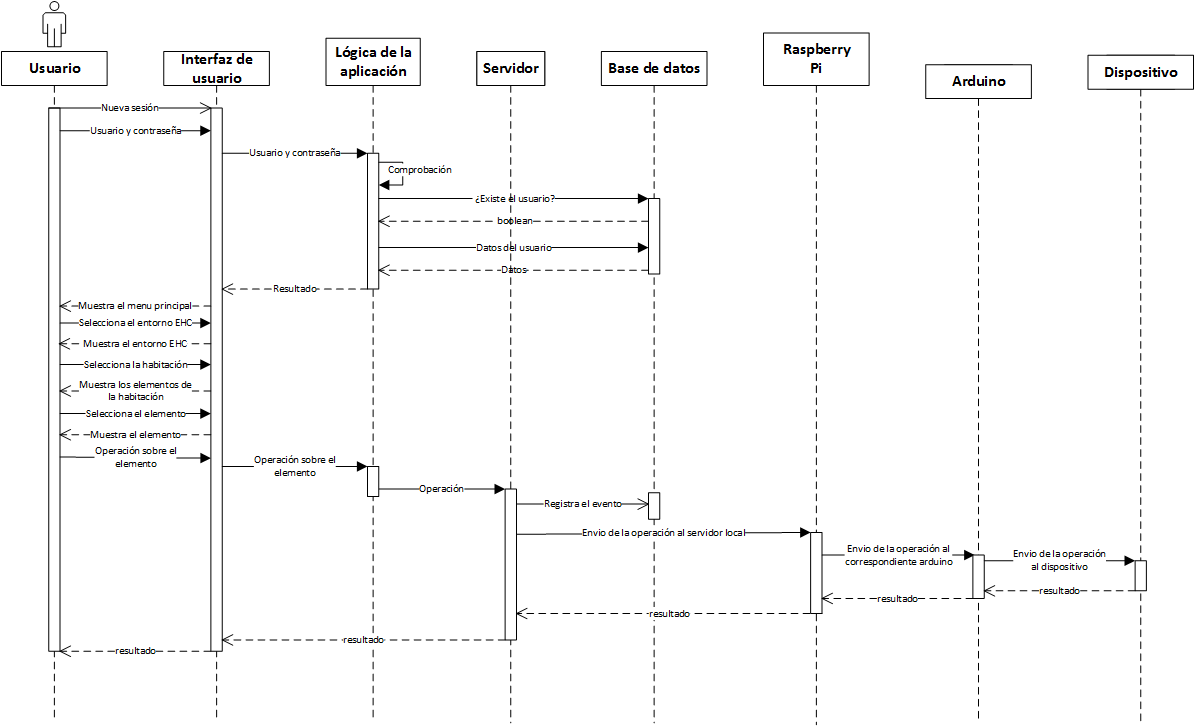
\includegraphics[width=0.9\textwidth]{4.Disenio/Imagenes/DisenioEHC}
	\caption{Diagrama de secuencia de la autentificaci\'on en el sistema y controlar un dispositivo.}
	\label{fig:diagramaSecuencia}
\end{figure}

\begin{figure}
	\centering
	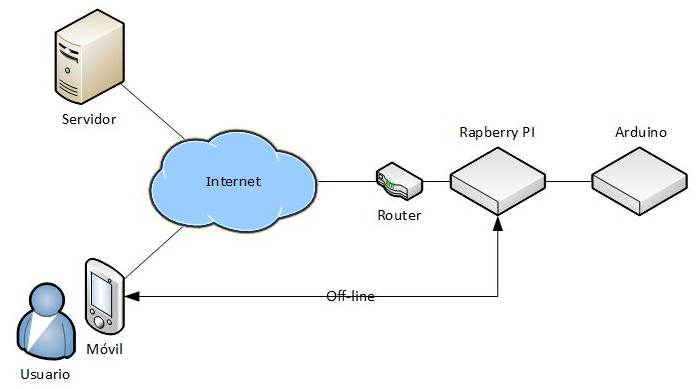
\includegraphics[width=0.8\textwidth]{4.Disenio/Imagenes/arquitectura}
	\caption{Arquitectura del sistema.}
	\label{fig:arquitectura}
\end{figure}


\begin{figure}
	\centering
	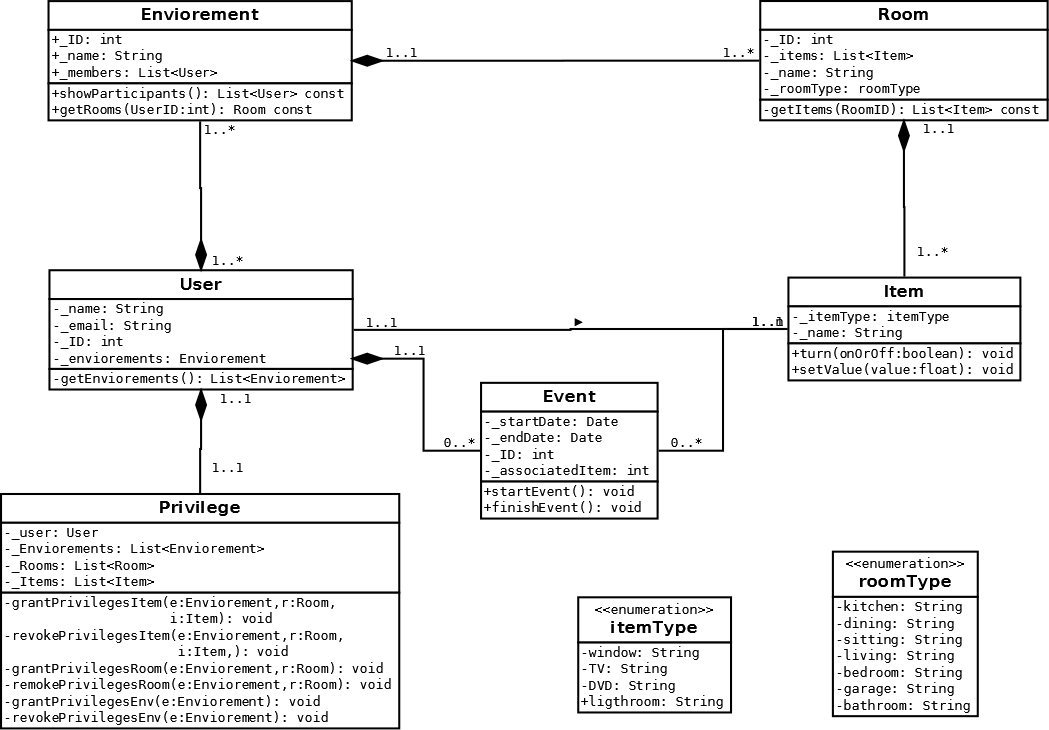
\includegraphics[width=0.8\textwidth]{4.Disenio/Imagenes/diagramaClase}
	\caption{Arquitectura del sistema.}
	\label{fig:diagramaClase}
\end{figure}



(Introducir diagrama de clases, diagrama de comunicacion y diagrama de secuencia)


\chapter{Vista de proceso}
El objetivo es mostrar que hace el sistema en alto nivel y toma en cuenta alguno de los ya citados requisitos no funcionales como es el rendimiento y la disponibilidad. Se describen tareas, sus interacciones y configuraciones, y la asignaci\'on de objetos del dise\~no y clases a las tareas. 
Este tipo de vista es fundamental para sistemas en el que el grado de concurrencia es elevado.
La arquitectura de procesos se describe en varios niveles de abstracci\'on donde cada uno de ellos tienen una funci\'on determinada.

(DIAGRAMA DE ACTIVIDAD)
\chapter{Vista de desarrollo}
Esta vista es fundamental como punto de partida para el equipo de desarrollo para saber como iniciar y organizar el código. El software quedará dividido en varios subsistemas (que a su vez están organizados en capas o jerarquías) que pueden ser desarrollados por uno o varios desarrolladores.

Para poder definir esta vista, previamente se ha tenido que identificar y definir todos los elementos del software.

(Incluir diagrama de paquetes y diagrama de componentes)

\begin{figure}
	\centering
	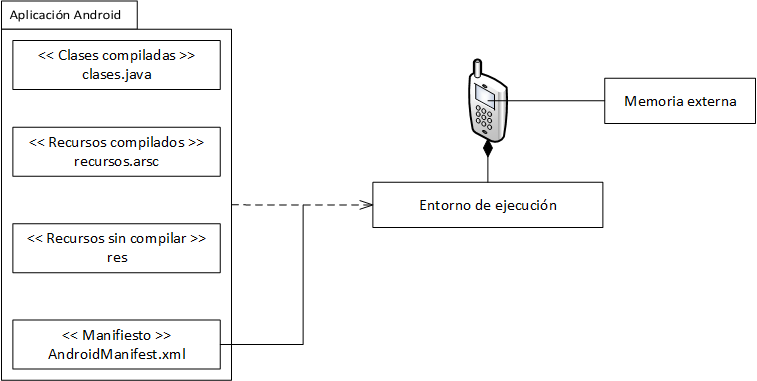
\includegraphics[width=0.65\textwidth]{4.Disenio/Imagenes/AppAndroid}
	\caption{Despliegue de la aplicación Android.}
	\label{fig:appAndroid}
\end{figure}

\chapter{Vista de implementación}

\section{Introducción}
Esta seccion describe la estructura general de la implementaicon del sistema. Muesta la descomposicion del sistema en subsistemas y cuales de estos son los mas importantes. Comprende a grandes rasgos todos aquellos artefactos que se utilizan para ensamblar el sistema y ponerlo en producción, ya listo para su distribución física

La arquitectura del sistema esta distribuida en 3 capas
\begin{enumerate}
\item Presentaci\'on: Esta constituida por todos aquellos componentes visibles para el usuario junto con pequeños submodulos de validacion de datos de entrada y salida. Los usuarios, podrán acceder a esta capa de presentación a través de las siguientes plataformas:
\begin{enumerate}
\item Web: podr\'an acceder a trav\'es de cualquier ordenador con conexi\'on local (si se encuentra en el entorno EHC) o por Internet.
\item M\'ovil: dispondr\'an tanto de una aplicaci\'on para iOS como para Android. A través de esta plataforma también es posible conectarse via local o via Internet.
\end{enumerate}
\item Aplicaci\'on: en esta capa englobamos todo aquello a la l\'ogica de la aplicaci\'on, además de proveer toda la lógica funcional para conectar la capa de presentación con la capa de transferencia de datos . 
\item Datos:   Esta capa consiste en una base de datos MYSQL que provee persistencia de datos. Se sirve de "procedimientos almacenados" que poseen acceso directo a los propipos datos de la base de datos con lo que se consigue fluidez y buena respuesta en la base de datos
    Esta capa se comunica con la capa de Servicio Web para responder a las peticions SQL.
\end{enumerate}


\section{Vista general del sistema}

La arquitectura del sistema está definida en la figura ~\ref{fig:arquitectura}. En dicha figura, podemos destacar los siguientes elementos y características:
\begin{itemize}
\item Dispositivo: el acceso al sistema EHC se puede realizar mediante:
\begin{itemize}
\item Dispositivo móvil: usando las aplicaciones disponibles tanto para iOS como para Android.
\item Ordenador: a través del portal EHC.
\end{itemize}
\item Servidor: será el encargado de enviar las peticiones del usuario a desde el dispositivo origen al entorno EHC a través de Internet. También será el encargado de almacenar toda la información requerida para el sistema.
\item Router: será necesario para poder almacenar la información del entorno EHC y para poder enviar/recibir peticiones a través de Internet.
\item Raspberry PI: funcionará como servidor local del entorno EHC. Será el encargado de gestionar las peticiones recibidas a través de la red local y/o de Internet hacia los dispositivos domotizados del hogar.
\item Arduino: es el subsistema encargado de controlar todos los sensores y actuadores instalados en un dispositivo.
\item Envio de peticiones: como ya se ha mencionado, estas peticiones pueden realizarse a través de Internet o a través de una red local donde estén conectados tanto el terminal origen como el servidor local.
\end{itemize}

\begin{figure}[h!]
	\centering
	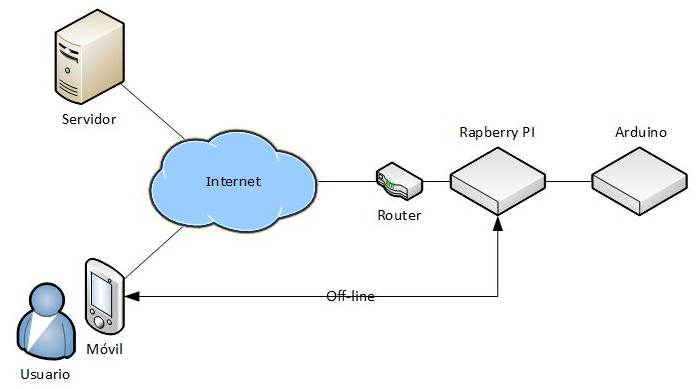
\includegraphics[width=0.8\textwidth]{4.Disenio/Imagenes/arquitectura}
	\caption{Arquitectura del sistema.}
	\label{fig:arquitectura}
\end{figure}


%%%%%%%%%%%%%%%%%%%%%%%%%%%%%%%%%%%%%%%%%%%%%%%%%%%%%%%%%%%%%%%%%%%%%%%%%%%%%%%%%%%

\chapter{Vista de datos}

El sistema atiende al siguiente diagrama relacional:


\begin{figure}[h!]
	\centering
	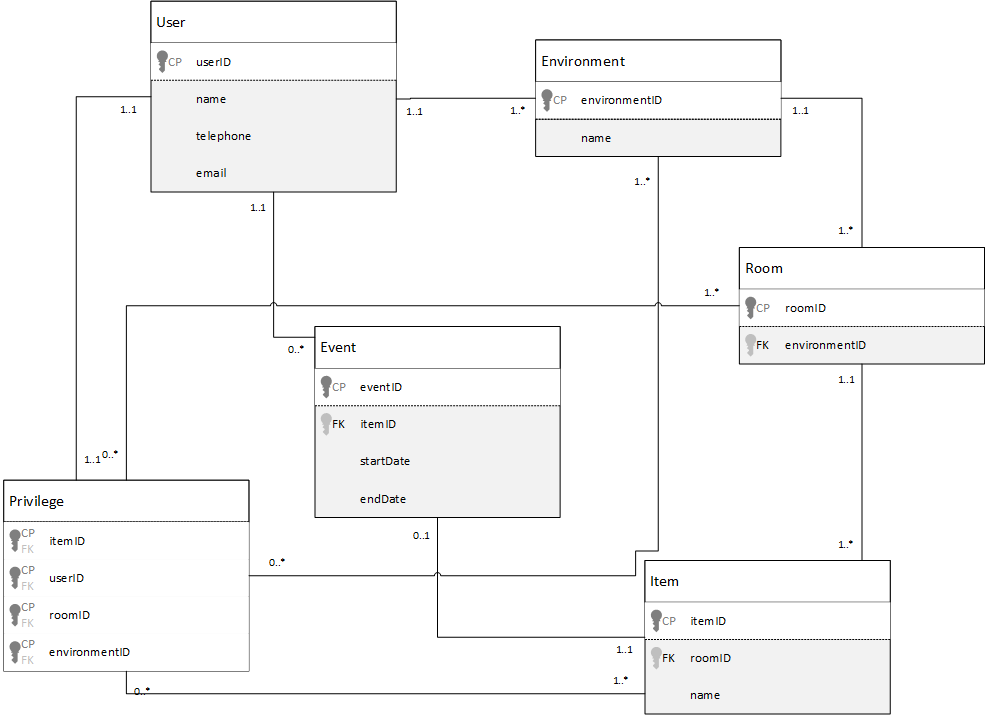
\includegraphics[width=0.8\textwidth]{4.Disenio/Imagenes/ER}
	\caption{Diagrama entidad-relación}
	\label{fig:ER}
\end{figure}








%Puesto que los requisitos de usuario son los mismo que los Funcionales, podriamos omitir las categorias ReqUsuario y ReqSistema y dar por hecho que son todos de sistema (Los de usuario estan expuestos en el documento Vision)


% % % % % % Fin del cuerpo
